	% Welcome! This is the unofficial University of Udine beamer template.

% We defined four theme colors: UniBrown, UniBlue, UniGold
% and UniOrange. For example, to write some uniud-brownish
% text, just use: \textcolor{UniBrown}{Hello!}

\documentclass[usenames,dvipsnames]{beamer}
\usepackage[utf8]{inputenc}
\usepackage{verbatim}
\usetheme{uniud}
%\bibliography{bib}
%%% Bibliography
%\usepackage[style=authoryear,backend=biber]{biblatex}
%\addbibresource{bib.bib}
\usepackage{tikz}
\usetikzlibrary{patterns,snakes}
%\DeclareNameAlias{author}{first-last}

%%% Suppress biblatex annoying warning
\usepackage{silence}
\WarningFilter{biblatex}{Patching footnotes failed}

%%% Some useful commands
% pdf-friendly newline in links
\newcommand{\pdfnewline}{\texorpdfstring{\newline}{ }} 
% Fill the vertical space in a slide (to put text at the bottom)
\newcommand{\framefill}{\vskip0pt plus 1filll}
\newcommand{\bigCI}{\mathrel{\text{\scalebox{1.07}{$\perp\mkern-10mu\perp$}}}}

\title[Blind Separation of Nonlinear Mixtures]{‌\vspace{0.5cm}\\
Blind Separation of Nonlinear Mixtures of Stochastic Processes}
\author[Behrad Moniri]{
  Behrad Moniri
  \pdfnewline
  \texttt{bemoniri@ee.sharif.edu}
  \pdfnewline\pdfnewline
    \textbf{Advisor}:\\ Prof. Massoud Babaie-Zadeh
}
\institute{\small{EE Department, Sharif University of Technology}}
\date{}
\begin{document}

\begin{frame}
\titlepage
\end{frame}

\begin{frame}{Outline}
\tableofcontents
\end{frame}


\section{Introduction to Blind Source Separation}
\begin{frame}
\frametitle{Blind Source Separation (BSS)}
\framesubtitle{Introduction}

\begin{figure}
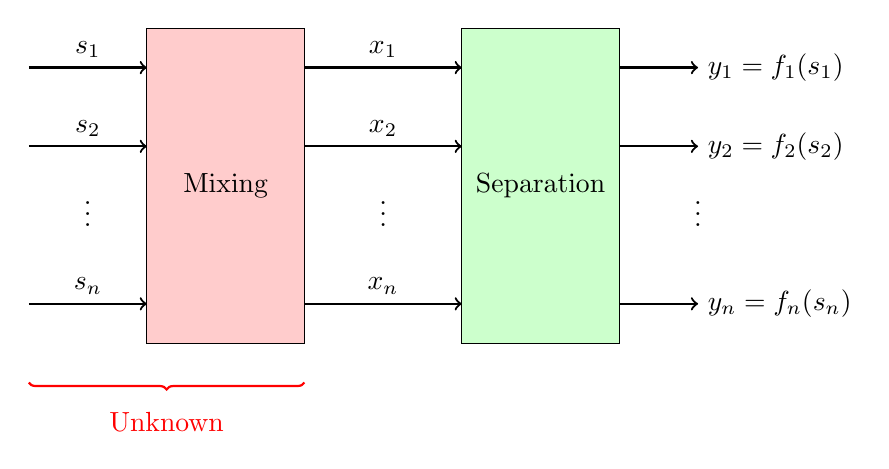
\begin{tikzpicture}

\onslide<1->{
\filldraw[draw = black, fill = red!20!white] (0,0) rectangle (2,4);
\node (text) at (1,2){Mixing};

\foreach \x in {0.5, 2.5, 3.5}
{
	\draw[->, thick] (-1.5, \x) -- (0, \x);
}

\node (vdotsin) at (-0.75,1.75){$\vdots$};


\node [anchor=south] (vdotsin) at (-0.75,0.5){$s_n$};
\node [anchor=south] (vdotsin) at (-0.75,2.5){$s_2$};
\node [anchor=south] (vdotsin) at (-0.75,3.5){$s_1$};


\foreach \x in {0.5, 2.5, 3.5}
{
	\draw[->, thick] (2, \x) -- (4, \x);
}

\node (vdotsin) at (3,1.75){$\vdots$};

\node [anchor=south] (vdotsin) at (3, 0.5){$x_n$};
\node [anchor=south] (vdotsin) at (3, 2.5){$x_2$};
\node [anchor=south] (vdotsin) at (3, 3.5){$x_1$};
}
\onslide<2->{
\filldraw[draw = black, fill = green!20!white] (4,0) rectangle (6,4);
\node (text) at (5,2){Separation};

\foreach \x in {0.5, 2.5, 3.5}
{
	\draw[->, thick] (6, \x) -- (7, \x);
}
\node (vdotsin) at (7,1.75){$\vdots$};

\node [anchor=west] (vdotsin) at (7, 0.5){$y_n = f_n(s_n)$};
\node [anchor=west] (vdotsin) at (7, 2.5){$y_2 = f_2(s_2)$};
\node [anchor=west] (vdotsin) at (7, 3.5){$y_1 = f_1(s_1)$};
}
\onslide <2->{
\draw [
red, thick,
decoration={
	brace,
	mirror,
	raise=0.5cm
},
decorate
] (-1.5, 0) -- (2, 0);

\node [red, anchor=north] at (0.25, -0.75){Unknown};

}
\end{tikzpicture}
\end{figure}
\end{frame}


\section{Review of the Previous Talk}
\begin{frame}
\frametitle{Linear and Non-Linear BSS}
\begin{alertblock}{Darmois-Skitovic Theorem \small{[Darmois-Skitovich ∼1950]}}
In the linear setting, the model is identifiable if the sources are \textbf{non-Gaussian} random variables.
\end{alertblock}
\pause
\begin{exampleblock}{Non-Linear Mixtures}
Non-linear mixtures are harder!
\small{
\begin{equation*}
\begin{cases}

S_1 = \mathrm{Rayleigh}(\sigma)\\
S_2 = \mathrm{Uniform} [0, 2\pi]
\end{cases}
\implies
X_1 = S_1 \cos (S_2) \perp \!\!\! \perp X_2 =  S_1 \sin (S_2)
\end{equation*}
}
\end{exampleblock}
\end{frame}
\normalsize


\begin{frame}
\frametitle{New Separability Results}
	\begin{alertblock}{Permutation Contrastive Separation [\footnotesize{Hyvarinen et al., 2017}]}
The mixture
		$\textbf{x}(t) = \textbf{f}\big(\textbf{s}(t)\big)$ is separable if:
		\begin{itemize}
			\item
			$\textbf{f}$ is invertible and smooth!
			\item
			$s_i(t)$:  \textbf{stationary},  \textbf{ergodic} and  \textbf{ \textit{uniformly dependent}}.
			\item
			$s_i(t)$ are not \textbf{ \textit{quasi-Gaussian}}.		
		\end{itemize}
	\end{alertblock}
	\begin{block}{Time Contrastive Learning \footnotesize[{Hyvarinen et al., 2016}]}
The mixture
$\textbf{x}(t) = \textbf{f}\big(\textbf{s}(t)\big)$ is separable if:
\begin{itemize}
\item
$
	\log p_\tau(s_i)=    \lambda_{i}(\tau) q(s_i) - \log Z( \lambda_{i}(\tau))
	\label{eq:p_tau_simple}
$
\item
$[\mathbf{L}]_{\tau, i} = 
	\lambda_{i, 1}(\tau) - \lambda_{i, 1}(1) \
	$
	has full column rank.
\end{itemize}
%	$$\Rightarrow \exists \mathbf{A} \in \mathbb{R}^{n\times n}
%	\;\;\; \exists\mathbf{d} \in \mathbb{R}^n
%	\;\;\;\;\;
%	q(\mathbf{s}_t) = \mathbf{Af^{-1}}(\mathbf{x}_t) + \mathbf{d}$$
\end{block}
\end{frame}

\section{Nonlinear BSS of Gaussian Processes}
\subsection{Theory}
\begin{frame}
\frametitle{Gaussianity Preserving Functions}
\textbf{A fundamental question:}

How can we separate Gaussian sources?

\pause
\begin{itemize}
\item Can nonlinear functions preserve Normality of random variables? \pause \textcolor{red}{YES!}

\begin{example}
Define the function $h$ as follows
\begin{equation*}
\label{E_CounterExampleOneDimensionalDiscontinued}
h(x)=
\begin{cases}
-x & a \leq |x| < b \\
x & \text{otherwise}
\end{cases}
\end{equation*}

If $X$ is a Normal Random variable, then $h(X)$ is also a Normal random variable.

\end{example}

\noindent
There are also many other examples! 

\pause
\item How about specific classes of functions?
\end{itemize}
\end{frame}

\begin{frame}
\frametitle{High Dimensional Polynomial Mappings}
\begin{itemize}
\item We have proved that a high dimensional polynomial function preserves normality, if and only if it is linear.
\end{itemize}

\begin{alertblock}{Polynomial Mixing Theorem}
	\label{T_MainTheoremGPs}
	
	Let $\mathbf{s} = (s_1, s_2, \dots, s_n)^\top \sim \mathcal{N} (\mu, \Sigma_s)$ be a vector of jointly normal random variables and ${\bf p}:\ \mathbb{R}^{n} \rightarrow \mathbb{R}^{n}$ be an invertible polynomial mapping.
	\begin{equation}
	\label{E_LinearPolynomial}
	{\bf y} = (y_1, y_2, \dots, y_n)^\top \triangleq{\bf p}({\bf s})
	\end{equation}
		
	The random variables $y_1,\dots,y_n$ are jointly normally distributed if and only if the polynomial $\bf {p}$ satisfies
	\begin{equation}
	\label{E_LinearPolynomial1}
	{\bf y}={\bf p}({\bf s})={\bf A}{\bf s}+{\bf b},
	\end{equation}
	where ${\bf A} \in \mathbb{R}^{n\times n}$ and ${\bf b} \in \mathbb{R}^n$.
\end{alertblock}
\end{frame}


\subsection{Algorithm}
\begin{frame}
\frametitle{Applications in Blind Source Separation}
Based on the previous theorem, we can prove the following corollary:

\begin{corollary}
	Let ${\bf x}(t) = {\bf f} ({\bf s}(t))$, where 
	\begin{itemize}
	\item
	${\bf f} : \mathbb{R}^n \to \mathbb{R}^n$ is an unknown invertible polynomial.
	\item 
	For all $i \in [n]$, $s_i(t)$ are mean zero Gaussian processes.
	\end{itemize}
If there exists polynomial ${\bf g} : \mathbb{R}^n \to \mathbb{R}^n$ such that ${\bf y} (t) = {\bf g}({\bf x}(t))$ are Gaussian Processes, then ${\bf h} = {\bf g} \circ {\bf f}$ is linear.
\end{corollary}
\end{frame}

\begin{frame}
\frametitle{Separation Algorithm}
A parametric model for polynomials:
\begin{equation*}
\label{E_Parametrizing}
{\bf g}({\bf x})=
\begin{bmatrix}
g_1({\bf x}) \\
g_2({\bf x}) \\
\vdots \\
g_n({\bf x})
\end{bmatrix}=
\begin{bmatrix}
\boldsymbol{\theta_1}\top \\
\boldsymbol{\theta_2}\top \\
\vdots \\
\boldsymbol{\theta_n}\top
\end{bmatrix}{\bf k}({\bf x})=
\boldsymbol{\Theta}{\bf k}({\bf x})
\end{equation*}

Calculate Neg-Entropy as a measure of Gaussanity:
\begin{equation*}
\label{E_NegEntropy}
\boldsymbol{\mathcal{J}}({ y_i})=\boldsymbol{H}({ \tilde{y}_i})-\boldsymbol{H}({ y_i})
\end{equation*}


Thus the algorithm should solve the following problem:
\begin{equation*}
\underset{\boldsymbol{\Theta}}{\min} \ \| \boldsymbol{\mathcal{J}}(\boldsymbol{\Theta}{\bf k}({\bf x})) \|_2^2
\end{equation*}
\end{frame}

\section{Simulations}
\begin{frame}
\frametitle{Simulations}
\small
Let $s_1, s_2 \sim \mathcal{N}(0,1)$ and $s_1 \bigCI s_2$.

\begin{equation*}
\label{E_SimulationMixture}
\begin{bmatrix}
s_1 \\
s_2
\end{bmatrix}
\rightarrow
\begin{bmatrix}
x_1 \\
x_2
\end{bmatrix}
=
\begin{bmatrix}
s_1+(s_1+s_2)^3 \\
s_2-(s_1+s_2)^3
\end{bmatrix}
\end{equation*}
This function can be exactly inverted as
\begin{equation*}
\label{E_SimulationInverseMixture}
\begin{bmatrix}
\hat{s}_1 \\
\hat{s}_2
\end{bmatrix}
=
\begin{bmatrix}
x_1-(x_1+x_2)^3 \\
x_2+(x_1+x_2)^3
\end{bmatrix}
\leftarrow
\begin{bmatrix}
x_1 \\
x_2
\end{bmatrix}.
\end{equation*}
\normalsize
\begin{figure}
\centering
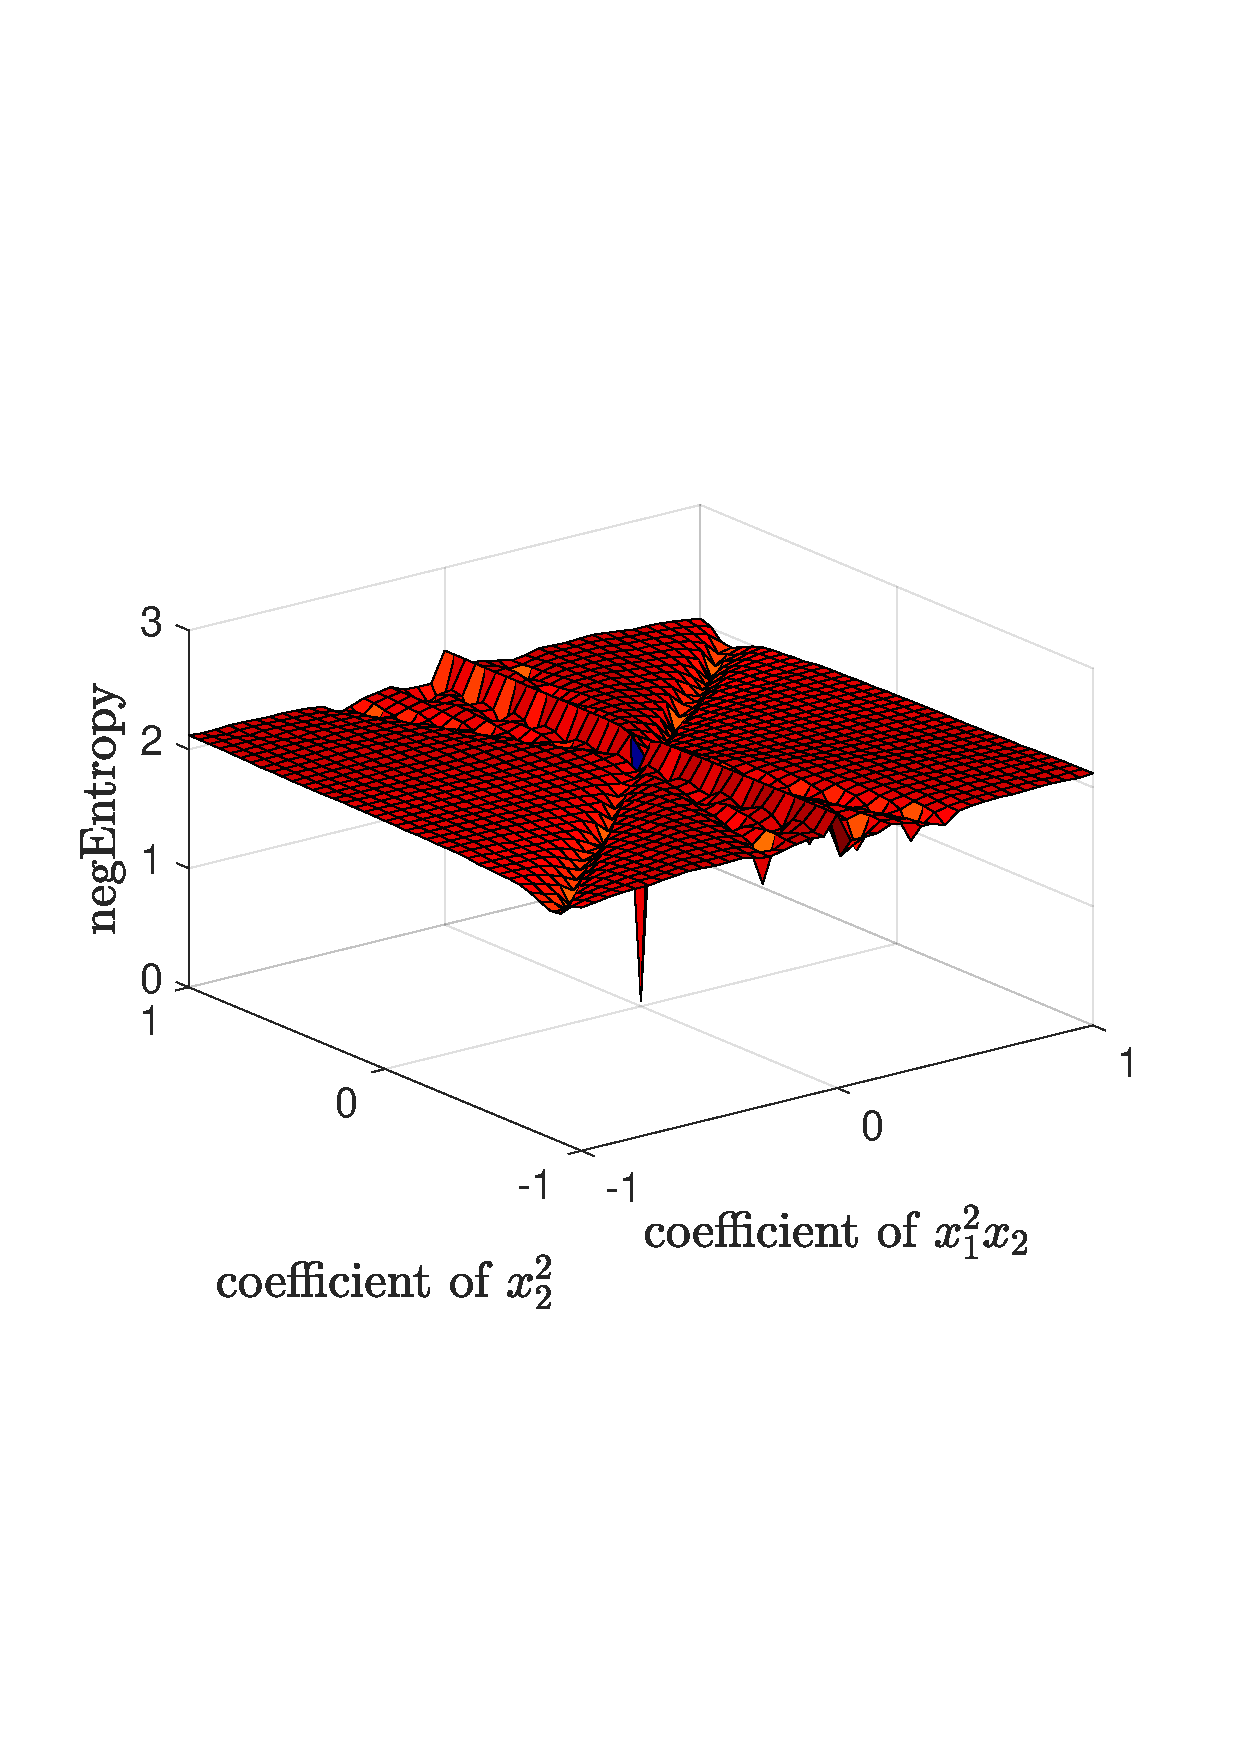
\includegraphics[trim={1cm 6cm 0.2cm 8.5cm},clip,width=0.5\linewidth]{Figures/2Dimensional_1.pdf}
\end{figure}

\end{frame}


\begin{frame}
\frametitle{Algebraic Functions and Rotations}

\begin{example}
	If $(X_1, X_2)^\top \sim \mathcal{N} \big(\mathbf{0}, \Sigma_X\big)$, then $Y_1 = \frac{X_1^2 - X_2^2}{\sqrt{X_1^2 + X_2^2}}$ and $Y_2 = \frac{2X_1 X_2}{\sqrt{X_1^2 + X_2^2}}$ is also a Gaussian random vector.
\end{example}
\pause
\begin{alertblock}{General Rotation Conjecture {[\small Eidlin, Linnik, Kagan}]}
	%\label{T_PreservingNorm}
	Let $\sigma > 0$ and
	Consider a random vector ${\bf x}=(x_1,x_2,\dots,x_n)^\top$ with every $x_j \sim \mathcal{N}(0,\sigma^2)$ and an algebraic transformation $\boldsymbol{\mathcal{A}}$.
	
	If ${\bf y}=\boldsymbol{\mathcal{A}}({\bf x})$ is normally distributed, then $\|{\bf y}\|_2=\|{\bf x}\|_2$.
\end{alertblock}

\end{frame}

\section{Future Works}

\begin{frame}
\frametitle{Ongoing Works}
\begin{itemize}
\item Gradual non-convexity methods for optimization.
\pause
\item Other measures of non-Gaussanity, e.g. 4th cumulants.
\pause
\item Can the Theorem 1 be extended to "polynomials" with positive and negative powers? 

{\color{red}\small{I believe the answer is positive and I think that the proof is not very difficult. But I am still working on this.}}
\pause
\normalsize
\item Finding two "good" sets of functions $\mathcal{F}$ and $\mathcal{G}$ such that $\forall f\in \mathcal{F} \;\; \forall g \in \mathcal{G}$, the function  $f\circ g $ is a polynomial. This will result in a new corollary and a new separation algorithm.

\end{itemize}
\end{frame}


\section{Bibliography}
\begin{frame}[t, allowframebreaks]
\frametitle{Selected Papers}
\scriptsize{
\bibliography{bib}
\nocite{shahram,TCL, PCL, newHyva, comon2010handbook, babaie2005general,linnik1968remark,kagan1973characterization, hyvarinen2000independent, ehsandoust}
\bibliographystyle{plain}
}
\end{frame}




\framecard{Thank You!}


\end{document}